\documentclass{beamer}
%\usepackage[utf8]{inputenc}
%\usepackage[T1]{fontenc}
\usepackage[french]{babel}
\usepackage{hyperref}
\usepackage{graphicx}
\usepackage{amsmath,amssymb}
\usepackage{tabularx}
\usepackage{booktabs}
\usepackage[compatibility=false]{caption}
\usepackage[toc,page]{appendix}
\usepackage{minted}

\newcolumntype{Y}{>{\centering\arraybackslash}X}

\usetheme[numbering=fraction,block=fill,progressbar=frametitle]{metropolis} %Use metropolis theme

\definecolor{bg}{rgb}{0.95,0.95,0.95}
\setminted{bgcolor=bg,fontsize=\scriptsize,autogobble,mathescape,breaklines,tabsize=2}
\setmintedinline{fontsize=\normalsize}

\begin{document}
%\setbeamertemplate{blocks}[rounded]
\title{Algorithmie - Complexité et structures de données}
\date[15 fév. 2017]{Mercredi 15 février 2017}
\author[nicolas.audebert@onera.fr]{Nicolas Audebert}
\institute{}
%\titlegraphic{\includegraphics[width=0.3\textwidth]{logo-ponts}}

\setmainfont{Fira Sans}
\maketitle


\AtBeginSection[]{
  \begin{frame}{Plan de la séance}
  \small \tableofcontents[currentsection, hideothersubsections]
  \end{frame}
}

\newcommand{\todo}[1]{\textbf{[TODO: #1]}}

\begin{frame}{Ressources, polycopié, TD, email}

\begin{block}{Ressources du cours}
    \begin{itemize}
    \item \textbf{Site web du cours :} \url{http://imagine.enpc.fr/~monasse/Algo}
    \item \textbf{Mes slides :} \url{https://nicolas.audebert.at/teaching/algo/}
    \end{itemize}
\end{block}

\begin{exampleblock}{Contact}
    \textbf{Email :} \href{mailto:nicolas.audebert@onera.fr}{nicolas.audebert@onera.fr}
\end{exampleblock}

\end{frame}

\section{Qu'est-ce que l'algorithmie ?}
\begin{frame}{Pourquoi ce cours ?}

\begin{block}{Introduction à la programmation C++}
Apprendre à manipuler le C++ comme outil.
\end{block}

\begin{block}{Algorithmie}
Apprendre à l'informatique comme discipline.
    \begin{itemize}
        \item Qu'est-ce qu'un algorithme ? Un bon algorithme ?
        \item Comment évaluer et comparer différents algorithmes ?
        \item Quels sont les algorithmes classiques pour mon problème ?
    \end{itemize}
\end{block}

\end{frame}

\begin{frame}{Algorithme}

\begin{block}{Qu'est-ce qu'un algorithme ?}
Un algorithme est une procédure comportant une suite finie d'opérations permettant d'obtenir un résultat à partir d'entrées connues.
\end{block}

\begin{block}{Propriétés d'un algorithme}
Un algorithme est une procédure :
    \begin{itemize}
        \item répétable (par un humain),
        \item finie (réalisable en temps borné),
        \item non-ambigüe (bien définie),
        \item travaillant sur des entrées spécifiées,
        \item produisant des sorties.
    \end{itemize}
\end{block}

\end{frame}


\section{Rappels sur les tableaux}

\begin{frame}{Les tableaux en C++}
En C++ les tableaux sont de taille fixe. Cette taille peut-être déterminée soit :
\begin{itemize}
    \item à la compilation (tableau \textbf{statique}),
    \item à l'exécution (tableau \textbf{dynamiques})
\end{itemize}
Les tableaux sont des structures difficiles à manipuler (gestion de la mémoire, mécanisme de copie inexistant, \dots).

\begin{exampleblock}{Pour simplifier}
Il est plus facile d'utiliser les vecteurs (\texttt{vector}) de la STL.
\end{exampleblock}

\end{frame}

\section{Complexité}

\subsection{Notion de complexité}

\begin{frame}{Notion de complexité}
    \begin{block}{Définition}
        La \textbf{complexité} d'un algorithme est une estimation du nombre d'opérations nécessaires à son exécution en fonction des \textbf{paramètres} caractéristiques du problème.
    \end{block}
    \begin{exampleblock}{Remarque}
        La complexité représente le comportement asymptotique de l'algorithme (lorsque les paramètres deviennent très grands).
    \end{exampleblock}
\end{frame}

\begin{frame}{Notion de complexité}
\begin{block}{Les types de complexité}
  \begin{itemize}
    \item La \textbf{complexité en temps} : le nombre d'opérations élémentaires constituant l'algorithme.
    \item La \textbf{complexité en espace} : le nombre de cases mémoires élémentaires occupées lors du déroulement de l'algorithme.
  \end{itemize}
\end{block}

\begin{exampleblock}{Remarque}
On s'intéresse généralement à la complexité dans le pire des cas et, plus rarement, à la complexité en moyenne.
\end{exampleblock}
\end{frame}

\begin{frame}{Notion de complexité}
\begin{exampleblock}{Remarques}
\begin{itemize}
\item La complexité en espace et en temps sont complémentaires :
  \begin{itemize}
  \item Stocker tous les résultats (grand espace mémoire)
  \item Calculer à chaque besoin (faible espace mémoire, peut être lent)
  \end{itemize}
\item En général, la complexité en espace n'est pas un problème et c'est le temps qui importe (par exemple, pour des applications temps réel).
\end{itemize}
\end{exampleblock}
\end{frame}


\begin{frame}[fragile]{Histogramme d'une image $W\times{H}$ : version rapide}
\begin{columns}
    \begin{column}{0.6\textwidth}
    \begin{minted}{c}
    // On stocke les 256 valeurs de l'histogramme 
    int histo[256];
    // Initialisation à 0
    for(int i=0; i<256; i++){
        histo[i] = 0;
    }
    // Parcours de l'image par colonne
    for(int x=0; x<image.width(); x++){
        for(int y=0; y<image.height(); y++){
            histo[image(x,y)]++;
        }
    }
    // Affichage de l'histogramme
    for(int i=0; i<256; i++){
        drawRect(i,0,1,histo[i])
    }
    \end{minted}
    \end{column}
    \begin{column}{0.4\textwidth}
    \begin{block}{Analyse}
        \textbf{Mémoire :}\\
        1 tableau de 256 cases\\
        \textbf{Temps :}\\
        $W\times{H}$ pixels visités
    \end{block}
    \end{column}
\end{columns}
\end{frame}

\begin{frame}[fragile]{Histogramme d'une image $W\times{H}$ : version lente}
\begin{columns}
    \begin{column}{0.65\textwidth}
    \begin{minted}{cpp}
    for(int i=0; i<256; i++){
        // Valeur i de l'histogramme
        int h = 0;
        // Parcours de l'image
        for(int x=0; x<image.width(); x++){
            for(int y=0; y<image.height(); y++){
                if(image(x,y) == c){
                    h++;
                }
            }
        }
        drawRect(c,0,1,h);
    }
    \end{minted}
    \end{column}
    \begin{column}{0.35\textwidth}
    \begin{block}{Analyse}
    \textbf{Mémoire :}\\
    Pas de tableau\\
    \textbf{Temps :}\\
    256 passages sur chaque pixel\\
    $\rightarrow 256\times{W}\times{H}$
    \end{block}
    \end{column}
\end{columns}
\end{frame}

\begin{frame}{Mesure de complexité}

\begin{block}{Bornes de complexité}
    Le nombre d'opérations élémentaires constituant un algorithme est souvent complexe à déterminer. Pour plus de commodité, on cherche un encadrement de celui-ci, i.e. $f$ telle que :
\begin{equation}
k_1 \times f(N) < \text{complexité} < k_2 \times f(N)
\end{equation}
\end{block}

\begin{block}{Notation}
    On utilise la notation $O(f(n_1, n_2, n_3, \hdots))$\\
    où $N = \{n_1, n_2, n_3, \hdots\}$ sont les paramètres caractéristiques du problème.
\end{block}
\end{frame}

\begin{frame}{Exemple de mesure de complexité}
\begin{exampleblock}{Histogramme rapide}
  \begin{itemize}
    \item Espace : $O(nombre\_couleurs)$
    \item Temps : $O(nombre\_pixels)$
  \end{itemize}
\end{exampleblock}

\begin{exampleblock}{Histogramme lent}
    \begin{itemize}
        \item Espace : $O(1)$
        \item Temps : $O(nombre\_pixels * nombre\_couleurs)$
    \end{itemize}
\end{exampleblock}
\end{frame}

\begin{frame}[fragile]{Notion de complexité : exemples simples}
\begin{exampleblock}{Parcours des éléments d'un tableau}
\begin{minted}{cpp}
// Utilisation d'un tableau type vector
// Tableau de taille $N$
for(int i=0; i<tab.size(); i++){
  cout << tab[i] << endl;
}
\end{minted}
on accède une fois à chaque case $\rightarrow$ complexité $O(N)$
\end{exampleblock}
\end{frame}

\begin{frame}[fragile]{Notion de complexité : exemples simples}
\begin{exampleblock}{Recherche (naïve) de l'unicité des éléments dans un tableau}
\begin{minted}{cpp}
// Unicité dans tab
vector<bool> unique(tab.size(),false);
for(int i=0; i<tab.size(); i++){
    for(int j=i+1; j<tab.size(); j++){
        if(tab[i]==tab[j]){
            unique[i] = unique[j] = true;
        }
    }
}
\end{minted}
deux parcours imbriqués $\rightarrow$ complexité $O(N^2)$
\end{exampleblock}
\end{frame}

\begin{frame}[fragile]{Exemple : le $n^e$ terme de la suite somme}
Le choix de l'implémentation dépend de l'application et influe beaucoup sur le temps de calcul.
\begin{columns}
    \begin{column}{0.5\textwidth}
    \begin{block}{Peu de mémoire}
    \begin{minted}{cpp}
    // Calcul à la volée
    int s = 0;
    for(int i=0; i<n; i++){
        s+= i;
    }
    \end{minted}
    Complexité $O(n)$.
    \end{block}
    \end{column}
    \begin{column}{0.5\textwidth}
    \begin{block}{Peu de temps}
    \begin{minted}{cpp}
    // Pré-calcul
    vector<int> pre(1000000000,0);
    for(int i=1; i<pre.size(); i++)
        pre[i] = i + pre[i-1];

    // Utilisation
    int s = pre[n];
    \end{minted}
    Complexité $O(1)$ (en utilisation).
    \end{block}
    \end{column}
\end{columns}
\end{frame}


\begin{frame}{Les grandes classes de complexité}
\begin{block}{Ordres de grandeur de complexité 1/2}
\begin{itemize}
\item $O(1)$ : \textbf{constant}, pas d'influence des grandeurs du problème. \\
\textit{Exemple} : accès à une case d'un tableau, somme de deux constantes.
\item $O(\log(n))$ : \textbf{logarithmique}, algorithmes rapides, pas besoin de lire toutes les données.\\
\textit{Exemple} : rechercher un élément dans un tableau trié.
\item $O(n)$ : \textbf{linéaire}, proportionnel au nombre d'éléments.\\
\textit{Exemple} : sommer tous les éléments d'un tableau.
\end{itemize}
\end{block}
\end{frame}

\begin{frame}{Les grandes classes de complexité}
\begin{block}{Ordres de grandeur de complexité 1/2}
\begin{itemize}
\item $O(n\log(n))$ : \textbf{linéarithmique}, de nombreux algorithmes ``rapides''.\\
\textit{Exemple} : Tri optimal, Fast Fourier Transform
\item $O(n^k)$ : \textbf{polynomiale}, acceptable pour des données petites (faible $n$) et des puissances faibles (petit $k$).\\
\textit{Exemple} : $O(n^2)$ tri naïf
\item $O(2^n)$ : \textbf{exponentielle}, utilisable en pratique seulement pour des petites dimensions.
\item $O(n!)$ : \textbf{factorielle}, inutilisable dès que $n$ dépasse la dizaine.
\end{itemize}
\end{block}
\end{frame}

\begin{frame}{Temps de calcul relatifs}
En supposant qu'une opération élémentaire prend 10 ns, pour $n = 50$:
\begin{itemize}
    \item $O(1)$ : 10 ns
    \item $O(\log(n))$ : 20 ns
    \item $O(n)$ : 500 ns
    \item $O(n\log(n))$ : 850 ns
    \item $O(n^{2})$ : 25 µs
    \item $O(2^n)$ : 130 jours
    \item $O(n!)$ : $10^{48}$ ans
\end{itemize}
\end{frame}


\begin{frame}[fragile]{Exemple : flouter une image}
\begin{columns}
\begin{column}{0.65\linewidth}
\begin{exampleblock}{Floutage}
\begin{minted}{cpp}
// Flouter une image $W\times{H}$ sur un rayon $r$
for(int i=r/2; i<W-r/2; i++){
  for(int j=r/2; j<H-r/2; j++){
    newIm[i,j] = 0;
      for(int k=i-r/2; k<i+r/2; k++){
        for(int m=j-r/2; m<j+r/2; m++){
          newIm[i,j] += im(k,m);
        }
      }
      newIm[i,j]/= r*r;
  }
}
\end{minted}
$\rightarrow$ complexité $O(W\times{H}\times{r^2})$
\end{exampleblock}
\end{column}
\begin{column}{0.35\linewidth}
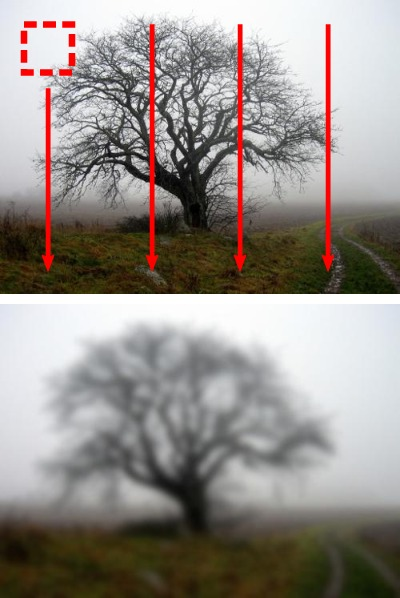
\includegraphics[width=\textwidth]{images/blur.pdf}
\end{column}
\end{columns}
\end{frame}


\begin{frame}{Classes de complexité}
\begin{block}{$P$ versus $NP$}
Les problèmes de classe $P$ sont les problèmes que l'on peut résoudre en temps polynomial.\\
Les problèmes de classe $NP$ sont ceux pour lesquels on ne connait pas de solution en temps polynomial.
\end{block}

\begin{exampleblock}{Example de problème $NP$}
Un commercial doit parcourir $N = \{n_1,\dots,n_k\}$ villes séparées par les distances $d_{i,j}$. Quelle est le chemin qui minimise la distance totale parcourue ?\\
Approche naïve : $O(n!)$, meilleur algorithme connu : $O(n^22^n)$.
\end{exampleblock}

\begin{alertblock}{Question à 1 000 000\$}
$P = NP$ ou $P \neq NP$ ?
\end{alertblock}
\end{frame}

\begin{frame}{En pratique\dots}
    \begin{block}{Relativisons !}
        \begin{itemize}
        \item Les complexités sont asymptotiques : elles sont valables pour les grandes tailles de données. 
        \item On omet généralement les constantes multiplicatives sont oubliées dans la notation $O()$.
        \end{itemize}
    \end{block}
    \begin{exampleblock}{Exemple}
        \begin{itemize}
            \item Algorithme A : $10^6\times{n} = O(n)$
            \item Algorithme B : $n^2 = O(n^2)$
            \item[$\rightarrow$] L'algorithme A est plus rapide ssi $n>10^6$
        \end{itemize}
    \end{exampleblock}
\end{frame}

\begin{frame}{Complexité en moyenne et dans le pire des cas}
    \begin{itemize}
        \item \textbf{Complexité moyenne} : caractérise le comportement attendu pour des répétitions sur des données aléatoires.
        \item \textbf{Complexité dans le pire des cas} : caractérise le comportement dans la pire configuration des données.
    \end{itemize}

\begin{exampleblock}{Importance}
L'application détermine le comportement important.
\begin{itemize}
\item \textbf{Complexité moyenne} : requêtes dans un moteur de recherche, traitement d'image.
\item \textbf{Complexité dans le pire des cas} :  applications critiques (aéronautique, \dots).
\end{itemize}
\end{exampleblock}

\end{frame}







\section{Structures de données}

\subsection{Vecteurs}


\begin{frame}{Le vecteur}
    \begin{block}{La classe}
    La classe est \mintinline{cpp}{std::vector} (simplement \mintinline{cpp}{vector} si on a utilisé \mintinline{cpp}{using namespace std}).\\
    Elle est \og templatée \fg, elle peut être utilisée pour contenir n'importe quel type de variable.
  \end{block}

\begin{exampleblock}{Avantages}
  \begin{itemize}
  \item Pas de mémoire à gérer
  \item Taille du vecteur connue grâce à la méthode \mintinline{cpp}{size()}
  \item La taille n'a pas besoin d'être connue dès le départ
  \end{itemize}
\end{exampleblock}
\end{frame}

\begin{frame}{Complexité de l'ajout d'un élément}

\begin{block}{Implémentation naïve}
    Quand on ajoute un élément avec la fonction \mintinline{cpp}{push_back()}, on redimensionne le tableau avec taille plus grande d'une case.
\end{block}

Ceci implique une recopie du tableau à chaque \mintinline{cpp}{push_back}.

\begin{exampleblock}<2>{Complexité}
    \centering
    $O(N)$
\end{exampleblock}
\end{frame}

\begin{frame}{Complexité de l'ajout d'un élément}
 \begin{block}{Implémentation maline}
 \begin{itemize}
     \item La taille du \mintinline{cpp}{vector} ne correspond pas la taille du tableau alloué.
    \item Quand on atteint la taille maximale du tableau, on réalloue en multipliant cette taille par un facteur $\alpha$.
 \end{itemize}
 \end{block}

 \begin{exampleblock}{Complexité}
     \centering
     $O(1)$ (en moyenne, $O(n)$ quand la taille maximale est atteinte)
 \end{exampleblock}
\end{frame}


\begin{frame}{Complexité moyenne du \texttt{push\_back} : preuve}
 
Supposons que l'on effectue $n$ ajouts par \mintinline{cpp}{push_back}.
 
\uncover<2->{Soit $k$ le nombre de redimensionnements. La taille du vecteur étant multipliée par $m$ à chaque fois, on a :
 $$ n < m^k \Rightarrow k \approx log_m(n)$$
 }
\uncover<3->{
Le nombre total de recopies est donc :
$$ \sum_{p=1}^k m^p = \sum_{p=1}^{log_m(n)} m^p = m \frac{m^{log_m(n)}-1}{m-1} = \frac{m\times n}{m-1}$$
}
\uncover<4->{
Le coût moyen (nombre de recopies / nombre d'ajouts) est alors :
    $$  \frac{m}{m-1} = O(1)$$
 }
\end{frame}

\begin{frame}{Propriétés des vecteurs}
    \begin{block}{Complexités des opérations sur les vecteurs}
  \begin{itemize}
  \item Lecture / Écriture : $O(1)$
  \item Ajout à la fin : $O(1)$
  \item Supression à la fin : $O(1)$
  \item Ajout à position donnée (\mintinline{cpp}{insert(it,val)}) : $O(N)$
  \item Suppression à position donnée (\mintinline{cpp}{erase(it)}) : $O(N)$
  \end{itemize}
\end{block}
\end{frame}

\subsection{Piles, files et listes}
\begin{frame}{La pile : \textit{Last In First Out} (LIFO)}
\begin{block}{Principe}
On ajoute et on retire les éléments un par un par le dessus.
\end{block}

\begin{exampleblock}{Implémentations}
\begin{itemize}
    \item \mintinline{cpp}{vector} (\mintinline{cpp}{include <vector>}) : \mintinline{cpp}{push_back(elem)}, \mintinline{cpp}{pop_back()}
    \item \mintinline{cpp}{stack} (\mintinline{cpp}{include <stack>}) : \mintinline{cpp}{push(elem)}, \mintinline{cpp}{pop()}
\end{itemize}
\end{exampleblock}

\begin{figure}[ht!]
  \centering
  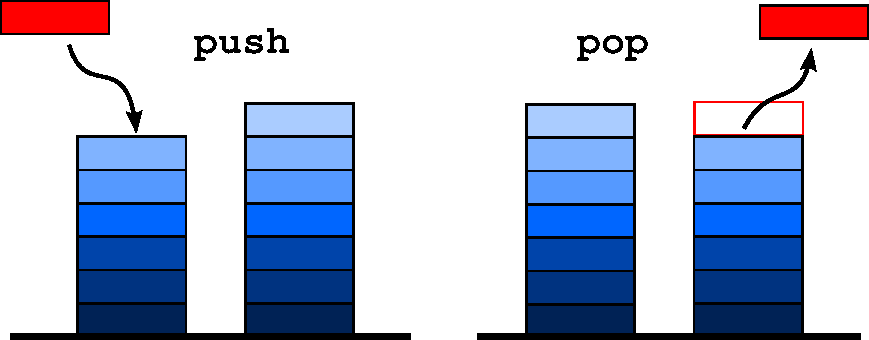
\includegraphics[width=0.5\linewidth]{./images/pile.pdf}
\end{figure}
\end{frame}



\begin{frame}{La file : \textit{First In First Out} (FIFO)}
\begin{block}{Principe}
On ajoute les éléments à l'arrière et on retire les éléments par l'avant.
\end{block}
\begin{exampleblock}{Implémentations}
Comme dans le cas de la pile : \texttt{push} et \texttt{pop}.
\end{exampleblock}

\begin{figure}[ht!]
  \centering
  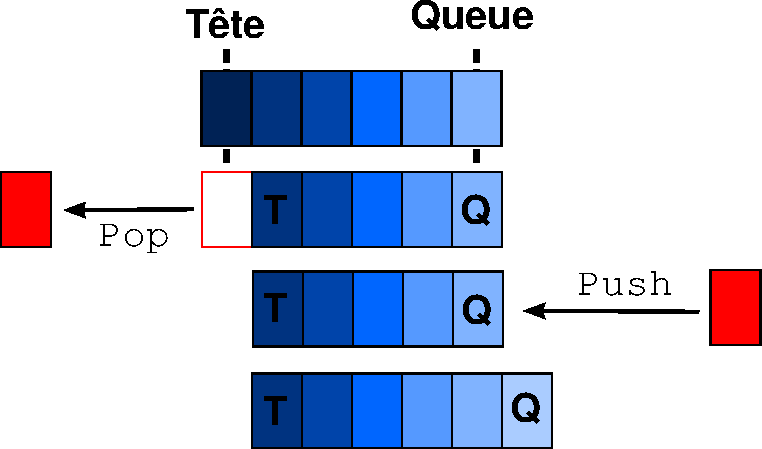
\includegraphics[width = 0.5 \linewidth]{./images/file.pdf}
\end{figure}

\end{frame}

\begin{frame}[fragile]{File : implémentation}
\begin{columns}
\begin{column}{0.5\linewidth}
    \begin{minted}{cpp}
    class File{
      std::vector<double> v;
      int debut, fin;
      int modulo(int i) const;
    public:
      File();
      bool empty();
      double front();
      void push(double d);
      double pop();
    };
    
    File::File(){
      debut= fin = 0 ;
    }
    \end{minted}
\end{column}
\begin{column}{0.5\linewidth}   
    \begin{minted}{cpp}
    bool File::empty() const {
      return (debut==fin) ;
    }
    
    // Tête de la file
    double File::front() const{
      return v[debut];
    }
    
    // Arithmétique modulo la taille de la file
    int File::modulo(int i){
      if(v.capacity()==0)
        return 0;
      return i%v.capacity();
    }
  \end{minted}
\end{column}
\end{columns}
\end{frame}

\begin{frame}[fragile]{File : implémentation}
\begin{columns}
\begin{column}{0.55\textwidth}
    \begin{minted}{cpp}
    // Ajout d'un élément
    void File::push(double d){
      int fin2 = modulo(fin+1);
      if(fin2==debut){
        std::vector<double> v2;
        for(int i=debut; i!=fin; i=modulo(i+1))
          v2.push_back(v[i]);
        v= v2;
        v.reserve(v.capacity()*2);
        debut = 0;
        fin2 = v.size()+1;
      }
      if(fin == v.size())
        v.push_back(d);
      else
        v[fin] = d;
      fin = fin2;
    }
    \end{minted}
\end{column}
\begin{column}{0.45\textwidth}
    \begin{minted}{cpp}
    // Retrait de l'élément de tête
    double File::pop(){
        double d = front();
        debut = modulo(debut+1);
        return d;
    }
    \end{minted}
\end{column}
\end{columns}
\end{frame}

\begin{frame}{File : propriétés}
\begin{block}{Complexité}
\begin{itemize}
  \item \texttt{push} : $O(1)$
  \item \texttt{pop} : $O(1)$
\end{itemize}
\end{block}

\begin{exampleblock}{Dans la STL}
  \begin{itemize}
  \item \texttt{queue} (\texttt{\#include <queue>}) : file
  \item \texttt{deque} (\texttt{\#include <deque>}) : \textit{double ended queue}
  \end{itemize}
\end{exampleblock}

\end{frame}


\begin{frame}
\frametitle{La liste chaînée}
Les structure vues précédemment ne sont efficaces que pour les ajouts en début ou en fin de tableau. Si on veut insérer ou supprimer au milieu du tableau, on utilise une \textbf{liste chaînée}.

\begin{block}{Structure}
Chaque maillon connait le maillon précédent et le maillon suivant.
\end{block}

\begin{figure}
\centering

\includegraphics[width=0.9 \linewidth]{./images/liste01.pdf}
\end{figure}
\end{frame}

\begin{frame}{La liste : insérer un élément}
\begin{block}{Idée}
Il suffit de modifier les indices des maillons précédents et suivants.
\end{block}

\begin{figure}
\centering
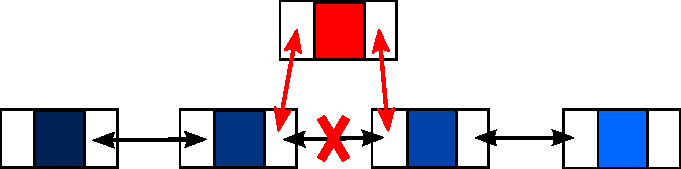
\includegraphics[width=0.9 \linewidth]{./images/liste02.pdf}
\end{figure}
\end{frame}

\begin{frame}{La liste : supprimer un élément}
\begin{block}{Idée}
On lie simplement les maillons précédents et suivants afin d'éviter le maillon à supprimer.
\end{block}

\begin{figure}
\centering
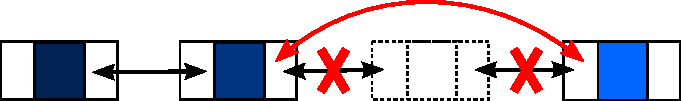
\includegraphics[width=0.9 \linewidth]{./images/liste03.pdf}
\end{figure}
\end{frame}

\begin{frame}[fragile]
\frametitle{La liste : implémentation}
On crée un tableau de maillons, ces maillons pointes sur les différentes cases du tableau.
\begin{minted}{cpp}
class Chainon{
  public:
    int prev, next;
    double value;
};
\end{minted}
\end{frame}

\begin{frame}[fragile]
\frametitle{La liste : implémentation - insertion}
On veut insérer l'élément $\text{elem}$ juste après l'indice $i$. Il est placé dans le tableau à la case d'indice $j$.
\begin{minted}{cpp}
t[j].val = elem; // assignation de elem dans la liste
t[j].prev = i;
t[j].next = t[i].next;
// t[j] est maintenant chaîné au successeur de t[i]
t[i].next = j;
// le nouveau successeur de t[i] est désormais t[j]
if(t[j].next != -1){
// Par convention, -1 signifie que l'élément suivant n'existe pas (fin de la liste)
  t[t[j].next].prev = j;
}
\end{minted}
\end{frame}

\begin{frame}[fragile]
\frametitle{La liste : implémentation - suppression}
\begin{minted}{cpp}
if(t[i].prev != -1){
  // On chaîne le prédécesseur s'il existe
  t[t[i].prev].next = t[i].next;
}
if(t[i].next !=-1){
  // On chaîne le successeur s'il existe
  t[t[i].next].prev = t[i].prev;
}
\end{minted}
\end{frame}

\begin{frame}
\frametitle{La liste : implémentation réelle}

\begin{block}{Pointeurs}
En pratique les champs \texttt{next} et \texttt{prev} sont des adresses mémoires, c'est-à-dire des pointeurs sur les chaînons.
\end{block}

\begin{exampleblock}{STL}
Implémentation standard : classe \texttt{std::list} (\texttt{\#include <list>}).
\end{exampleblock}

\end{frame}

\subsection{Les itérateurs}

\begin{frame}[fragile]
\frametitle{Les itérateurs}
Les itérateurs sont des éléments de la \textbf{STL}, qui permettent de parcourir les structures comme les listes, les piles, les files, les vecteurs, \dots

Ainsi si une pile ne donne accès qu'au premier élément, on peut quand même parcourir tout les éléments.

\begin{minted}{cpp}
vector<double>::iterator it = vect.begin();
vector<double>::const_iterator it2 = vect.begin();
for(; it != vect.end(); it++){
  *it = 10;
}
for(; it2 != vect.end(); it2++){
  cout << *it2 << endl;
}
\end{minted}
\end{frame}

\subsection{Récapitulaif}

\begin{frame}{Récapitulatif des complexités}
\begin{center}
\begin{tabular}{ c | c | c | c | c }
& vecteur & pile & file & liste\\
\hline
push\_back & $O(1)$ & $O(1)$ & $O(1)$ & $O(1)$\\
\hline
pop\_back & $O(1)$ & $O(1)$ & - & $O(1)$\\
\hline
push\_front & $O(N)$ & - & - & $O(1)$\\
\hline
pop\_front & $O(N)$ & - & $O(1)$ & $O(1)$\\
\hline
tab[i] & $O(1)$ & - & - & $O(N)$\\
\hline
insert & $O(N)$ & - & - & $O(1)$\\
\hline
erase & $O(N)$ & - & - & $O(1)$\\
\hline
\end{tabular}
\end{center}
\end{frame}

\subsection{Autres structures}

\begin{frame}{Autres structures classiques}
\begin{itemize}
\item \texttt{set} : un ensemble dans lequel un élément ne peut-être présent qu'une fois
\item \texttt{map} : associe à un élément une clé qui permet de le retrouver rapidement ($simeq$ dictionnaires Python)
\item \texttt{hashmap} : similaire à une \texttt{map}, mais les élément sont indexés avec une fonction de hachage pour accélérer les temps d'accès.
\item La file de priorité : files dont les éléments sortent par ordre de priorité.
\item Les graphes : généralisation des listes chaînées (réseaux, arbres de dépendances, \dots)
\end{itemize}
\end{frame}

\end{document}

